\documentclass[text.tex]{subfiles}

\begin{document}
\section{Cataloging Voronoi polygons for single general window}
The step from cataloging Voronoi polygons for a single rhombic window to cataloging Voronoi polygons for a single general window is significantly larger than the step from generating finite sections for a rhombic window to a general window described in the previous section. 

The goal is again to generate all possible finite sections of the quasicrystal with a general window that cover a circle of the covering radius. 

For that an opposite of the hyper-quasicrystal needs to be defined. To given general window $\Omega$ a rhombic window $\uwidehat{\Omega}$ is inscribed. Therefore $\uwidehat{\Omega}\subset\Omega$. The window $\uwidehat{\Omega}$ is called the hypo-window and the quasicrystal $\quasi{\uwidehat{\Omega}}$ is called the hypo-quasicrystal. 
$$\uwidehat{\Omega}\subset\Omega\subset\widehat{\Omega} \quad \Rightarrow \quad \quasi{\uwidehat{\Omega}}\subset\quasi{\Omega}\subset\quasi{\widehat{\Omega}}$$
The hypo-quasicrystal creates a subset of the quasicrystal and the hyper-quasicrystal creates a superset. In other words the points of the hypo-quasicrystal are always present in the quasicrystal and the presence of the points of the hyper-quasicrystal needs to be decided. That is the key idea for the algorithm. 

\begin{remark}
One-dimensional hyper-window means a one-dimensional window of the same size as is the size of the two-dimensional rhombic hyper-window. Equivalently for the hypo-window. 
\end{remark}

\begin{enumerate}
\item estimate the covering radius from the hypo-quasicrystal (it is certainly larger there than for the quasicrystal)
\item estimate the sufficient $n$ so that the finite section of the word of the hyper-quasicrystal covers the necessary distance
\item generate finite sections of the hyper-quasicrystal from the language of the sufficient $n$
\item mark the points of the hypo-quasicrystal in each finite section
\item determine which of the unmarked points belong to the quasicrystal
\item construct Voronoi polygons
\item select Voronoi polygons that actually appear in the quasicrystal
\end{enumerate}

\subsection{Identifying the points of the hypo-quasicrystal}
To take advantage of the hypo-quasicrystal it's points need to be identified in the finite sections. The one-dimensional quasicrystal corresponding to the hypo-quasicrystal is a sparser subset of the one-dimensinal quasicrystal corresponding to the hyper-quasicrystal. 

The identification is started already while generating the language $\mathcal{L}_\ell(n)$. The algorithm for dividing a one-dimensional window is augmented. Output of the new algorithm is no longer a section of the word of the quasicrystal, every second letter is $t_{2i}\in\{0,1\}$ and denotes whether the point after the distance represented by the previous letter is present in the one-dimensional quasicrystal corresponding to the hypo-quasicrystal. 

At each step of the iteration the intervals are further divided by the one-dimensional hypo-window. As is presented in Figure \ref{pic:twoWindowsIteration}.

\begin{figure}
\begin{center}
\begin{tikzpicture}

\coordinate (xc) at (0,0);
\coordinate (xa) at (15*0.3301270191,0);
\coordinate (xb) at (15*0.4641016151,0);
\coordinate (xd) at (15*0.5980762115,0);

\node [above] at (xc) {$c$};
\node [above] at (xa) {$a^\Omega$};
\node [above] at (xb) {$b^\Omega$};
\node [above] at (xd) {$d$};

\node [above] at (1,1) {$c'$};
\node [above] at (6,1) {$d'$};

% guide lines
\draw [dashed, ultra thin, opacity=0.6] (xc) -- (xa) -- (15*0.598076,-1) -- (15*0.267949,-1) -- cycle;
\draw [dashed, ultra thin, opacity=0.6] (15*0.330127, 0) -- (15*0.464102, 0) -- (15*0.267949,-1) -- (15*0.133975,-1) -- cycle;
\draw [dashed, ultra thin, opacity=0.6] (15*0.464102, 0) -- (15*0.598076, 0) -- (15*0.133975,-1) -- (0,-1) -- cycle;

\foreach \x in {0,...,1}
{
\draw [|-|] ($(xc)+(0,-\x)$) -- ($(xd)+(0,-\x)$);
\draw [fill] ($(xc)+(0,-\x)$) circle [radius=0.1];
\draw [fill] ($(xa)+(0,-\x)$) circle [radius=0.1];
\draw [fill] ($(xb)+(0,-\x)$) circle [radius=0.1];
\draw [fill=white] ($(xd)+(0,-\x)$) circle [radius=0.1];
}

\draw [dashed,ultra thin] (1,1) -- (1,-1);
\draw [dashed,ultra thin] (6,1) -- (6,-1);

\draw [-] (1,1) -- (6,1);
\draw [fill] (1,1) circle [radius=0.1];
\draw [fill=white] (6,1) circle [radius=0.1];


\node [below] at (0.5,0)            {\texttt{D0}};
\node [below] at (2.97595264325,0)  {\texttt{D1}};
\node [below] at (5.47595264325,0)  {\texttt{B1}};
\node [below] at (6.48076211325,0)  {\texttt{B0}};
\node [below] at (7.9663336995,0)   {\texttt{C0}};

\node [below] at (0.5,-1)           {\texttt{C0D0}};
\node [below] at (1.5048125,-1)     {\texttt{C0D1}};
\node [below] at (2.5336725,-1)     {\texttt{B1D1}};
\node [below] at (3.5384775,-1)     {\texttt{B0D1}};
\node [below] at (4.4855701,-1)     {\texttt{D0D1}};
\node [below] at (5.1855701,-1.17)     {\texttt{\dots}};

\end{tikzpicture}
\end{center}
\caption{Illustration of creating words with the marks of belonging to the one-dimensional hypo-window. The one-dimensional hypo-window is displayed as the interval $[c',d')$ and the one-dimensional hyper-window is displayed as the interval $[c,d)$. } 
\label{pic:twoWindowsIteration}
\end{figure}

Once constructing the finite sections of the quasicrystal, points are marked once both letters are succeeded by \texttt{1}. Finite section in Figure \ref{fig:showPotential} was created from the following words.
\begin{center}\texttt{D0B0D0C0D0D1C0D0D1C0} and \texttt{C0D0B1D0B0D1C0D0D1C0}\end{center}
The first letter is skipped and so the second letter determines the mark for the first points in the finite section. Therefore is the finite section smaller than with a rhombic window in previous section. 

The set of unmarked points $P = \quasi{\widehat{\Omega}}\setminus \quasi{\uwidehat{\Omega}}$ is called the potential of the finite section. 

\begin{figure}[h!]
\centering
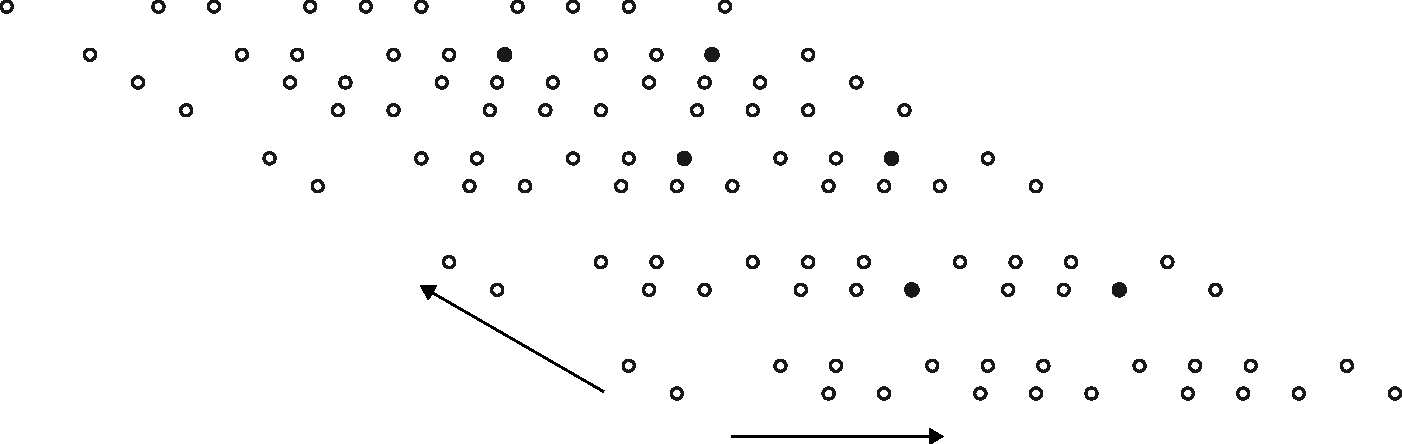
\includegraphics[width=0.7\textwidth]{catalogGeneral/showPotential}
\caption{Finite section created from the words \texttt{D0B0D0C0D0D1C0D0D1C0} (horizontal) and \texttt{C0D0B1D0B0D1C0D0D1C0} (vertical). The points of the hypo-quasicrystal (full) and the potential (empty).}
\label{fig:showPotential}
\end{figure}

The next step is to determine which points of the potential belong to the quasicrystal $\quasi{\Omega}$. In other words creating finite sections of the quasicrystal with a general window.

\subsection{Finite sections of a quasicrystal with a general window}
To acquire finite sections of the quasicrystal with a general window form the finite sections of the hypo-quasicrystal and their potential, they are precessed one by one. 

Let $F$ be the finite section and $P\subset F$ is it's potential. Clearly $F\setminus P$ are the points of the hypo-quasicrystal and $(F\setminus P)^\ast \subset \uwidehat{\Omega}\subset\Omega$.

The points of the potential are considered one at a time. For each $x\in P$ it needs to be tested whether $((F\setminus P)\cup x)^\ast$ fits inside the window $\Omega$. Method for such test was already covered in previous section.
$$(F\setminus P) = \{x_1,\dots,x_k\}$$
$$x^\ast\in\Omega \quad\wedge\quad x_i^\ast\in\Omega \quad\forall i\in\hat{k}$$
$$q_i = x_i - x \quad\forall i\in\hat{k}$$
$$x^\ast\in\Omega \quad\wedge\quad x^\ast+q_i^\ast\in\Omega \quad\forall i\in\hat{k}$$
$$x^\ast\in\Omega \quad\wedge\quad x^\ast\in\Omega-q_i^\ast \quad\forall i\in\hat{k}$$
$$x^\ast\in\bigcap\limits_{i\in\hat{k}}(\Omega-q_i^\ast)\cap\Omega$$
Therefore the test turns into whether is the intersection empty or not. If it is empty $x$ is removed from both $P$ and $F$ if it is not empty $x$ is only removed from $P$, thus becoming the point of the finite section $F\setminus P$. 

However the algorithm needs to test the fit for each subset of the potential. The algorithm therefore branches into a tree structure, one branch for every remaining point of the potential. The computational complexity is huge. 

Such process produces a superset of all finite sections of the algorithm, such finite sections that could appear in the quasicrystal. The next section presents a method of determining which finite sections actually do appear. 

\subsection{Voronoi polygons that actually appear in the quasicrystal}
The Figure \ref{fig:twoTiles} illustrates the issue nicely. Both finite sections are results from the algorithm from the previous section. Depending on the shape of the window the second one may fit in the window every time the first one does. That would imply that the first polygon never appears in the quasicrystal since it would always be cut to the smaller second one. 
\begin{figure}[h!]
\centering
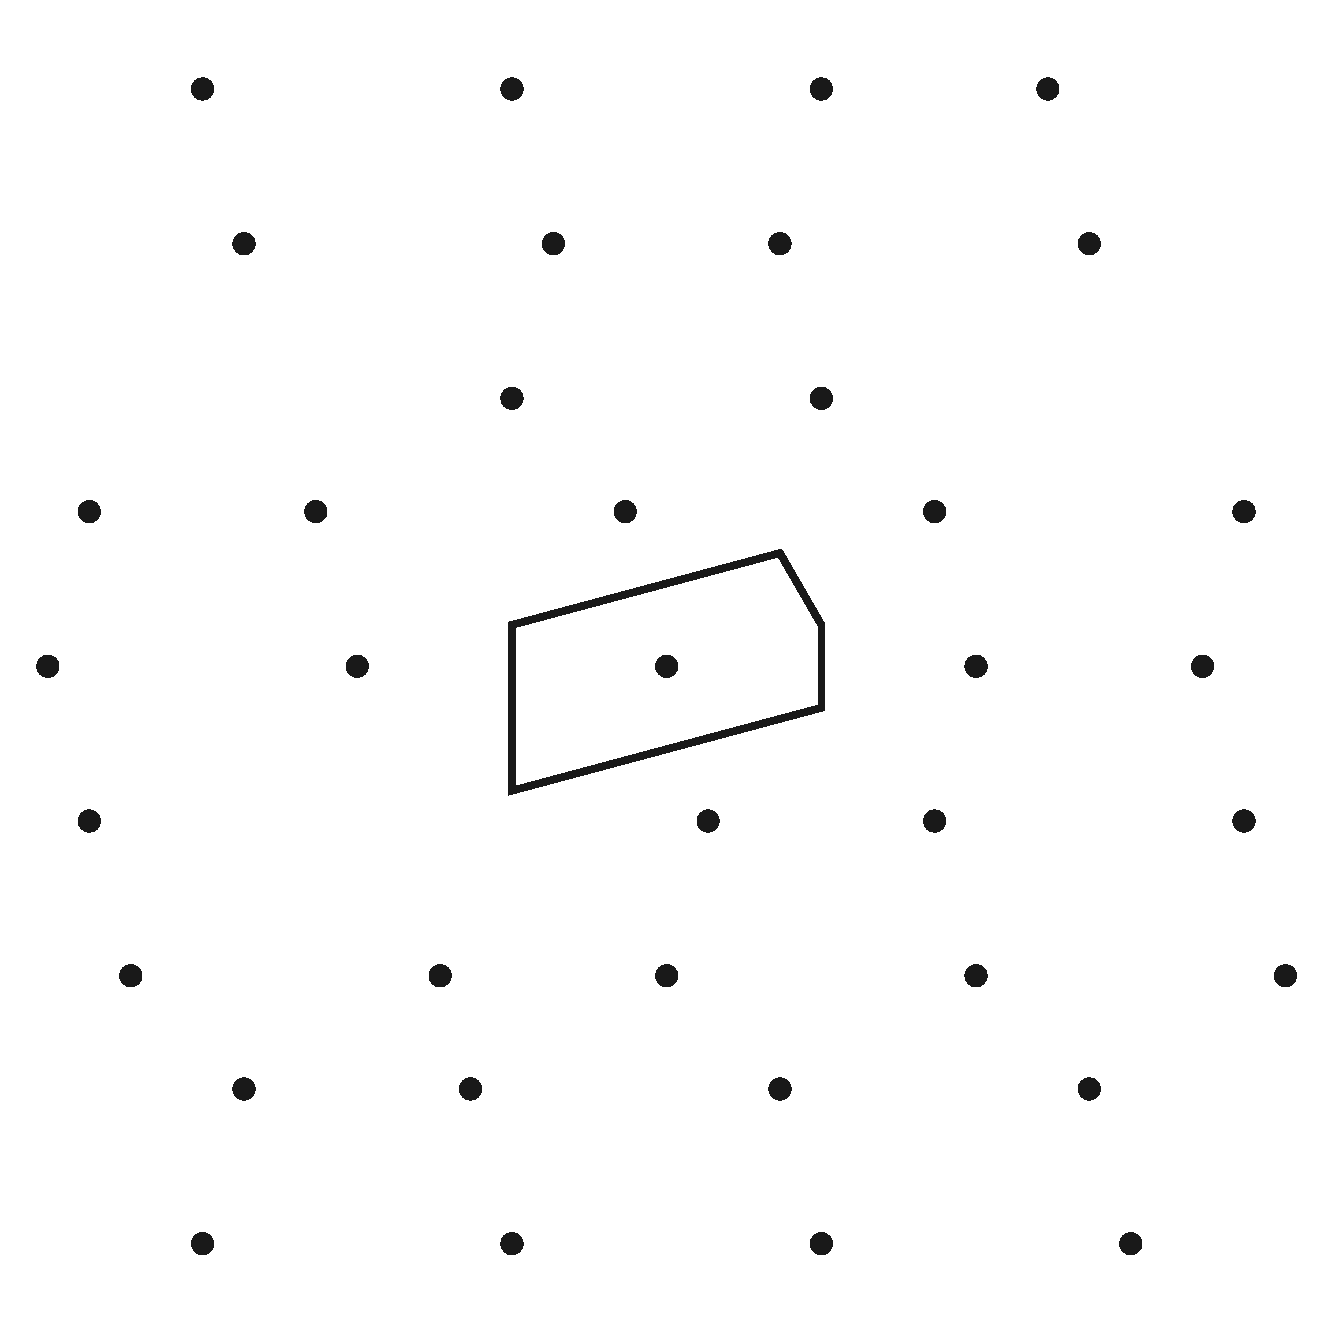
\includegraphics[width=0.4\textwidth]{catalogGeneral/tile00017}%
\qquad%
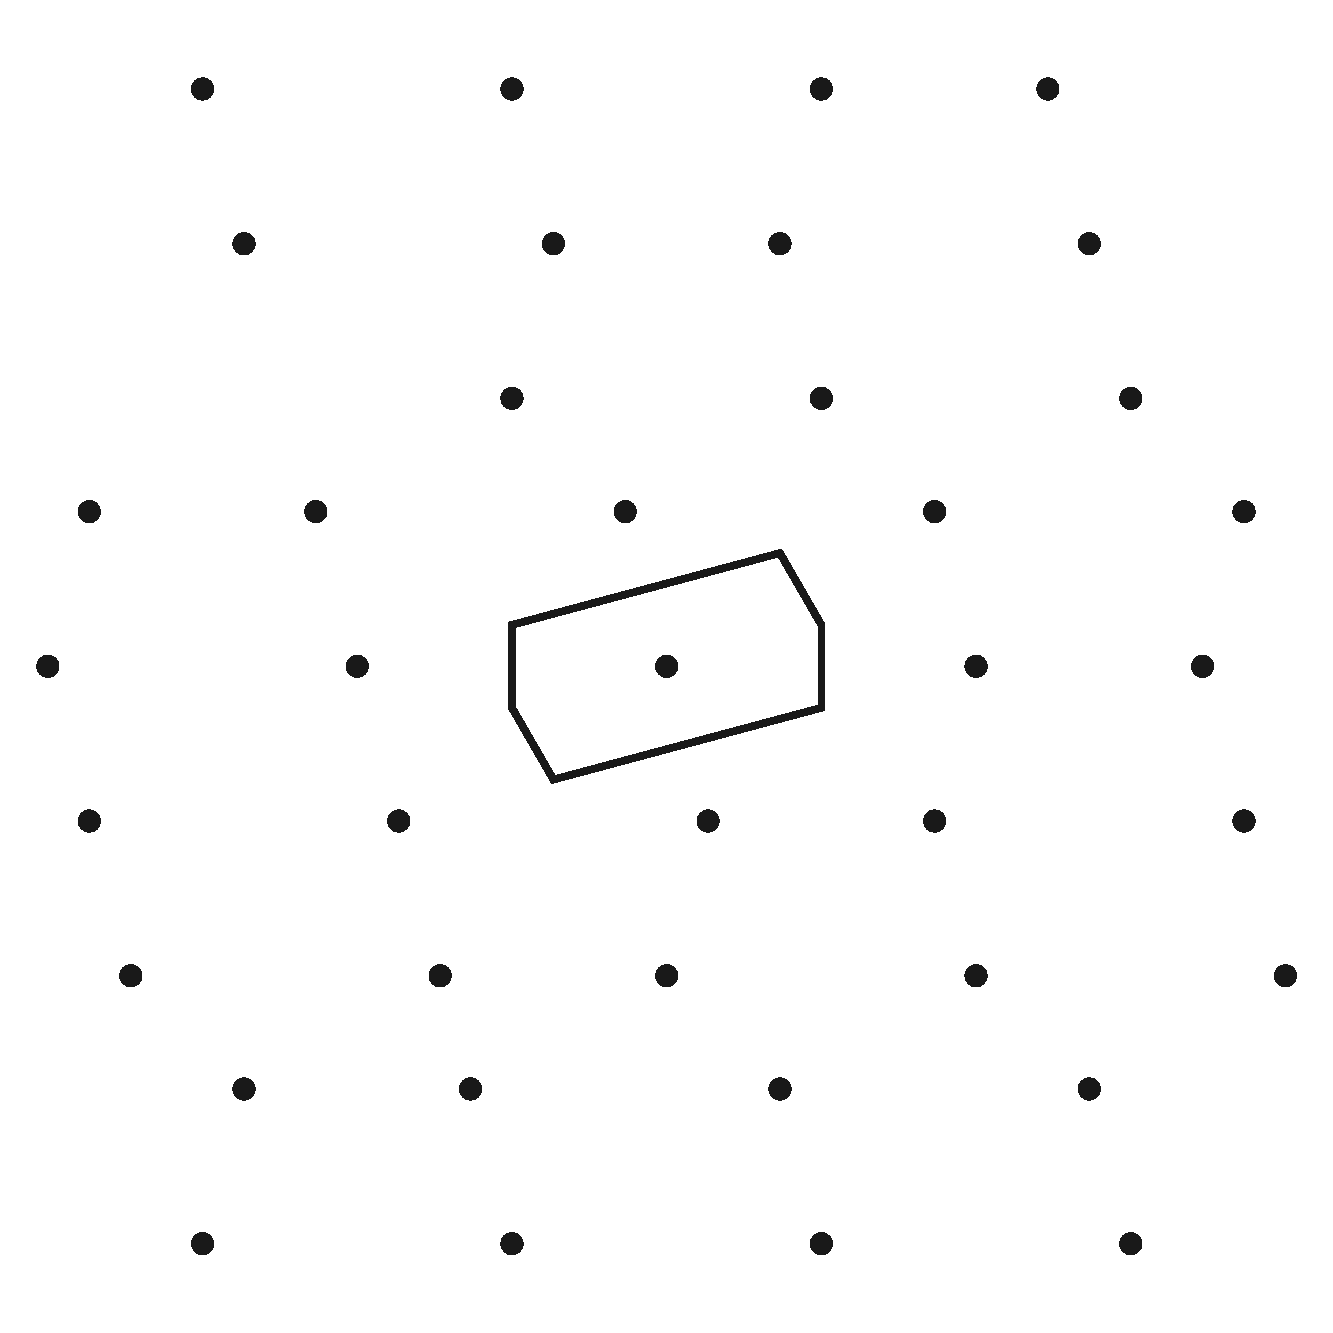
\includegraphics[width=0.4\textwidth]{catalogGeneral/tile00018}
\caption{Example of two Voronoi polygons constructed over two finite sections from the algorithm from the previous section.}
\label{fig:twoTiles}
\end{figure}

Solution was also partially covered while analyzing the quasicrystals with a rhombic window. 

Once a Voronoi polygon is created for each finite section only the domain of the polygon is kept and the rest is discarded. 

The intersection is constructed as before:
Let $V$ be one of the Voronoi polygons in the quasicrystal, $c$ the center of $V$, $D = \{p_1,\dots,p_k\}$ the domain of $V$ and $q_i = p_i - c$, $i\in\hat{k}$.
$$Q = \bigcap\limits_{i\in\hat{k}}(\Omega-q_i^\ast)\cap\Omega$$
Once $c^\ast\in Q$ then the domain of $V$ appears in the quasicrystal. For different Voronoi polygons these intersections may overlap. However unlike with a rhombic window, with a general window some intersections may get entirely covered by intersections of other Voronoi polygons and thus eliminating the corresponding Voronoi polygon from the quasicrystal. 

To determine which Voronoi polygons actually appear in the quasicrystal the intersection of all candidate Voronoi polygons need to be stacked up sorted from the smallest Voronoi polygon on the top and the polygons whose intersections are entirely coved are eliminated. Thus a catalog of Voronoi polygons for single quasicrystal with a general window is created. 
\end{document}
